\documentclass[12pt]{article}
\usepackage[utf8]{inputenc} % For UTF-8 encoding
\usepackage{amsmath, amssymb, amsthm} % For mathematical formatting
\usepackage{multirow} % For multirow in tables
\usepackage[a4paper, margin=0.75in]{geometry} % For setting page size and margins
\usepackage{xcolor, listings} % For code highlighting
\usepackage{longtable} % For long tables
\usepackage{graphicx} % For including images
\usepackage{float} % For better control of floating environments
\setlength{\parindent}{0pt}

% Define a custom float placement for stricter positioning
\floatplacement{table}{H}
\floatplacement{figure}{H}

\title{Computer Architecture HW 2}
\author{111062117, Hsiang-Sheng Huang}

\begin{document}

\maketitle

\section*{1}

\subsection*{(a)}

\begin{table}[H]
    \centering
    \begin{tabular}{|c|c|c|c|}
    \hline
    Subroutine Name & Starting Memory Address & Ending Memory Address & Reference \\
    \hline
    \textbf{iter\_fibonacci} & 0x0000 0000 0000 00b0 & 0x0000 0000 0000 00db &  jal ra, 0xb0 \\
    \hline
    \textbf{recur\_fibonacci} & 0x0000 0000 0000 00b0 & 0x0000 0000 0000 00e3 & jal ra, 0xb0 \\
    \hline
    \end{tabular}
\end{table}

\begin{table}[H]
    \centering
    \begin{tabular}{|p{2cm}|c|c|}
    \hline
    & \textbf{iter} & \textbf{recur} \\
    \hline
    main reference & 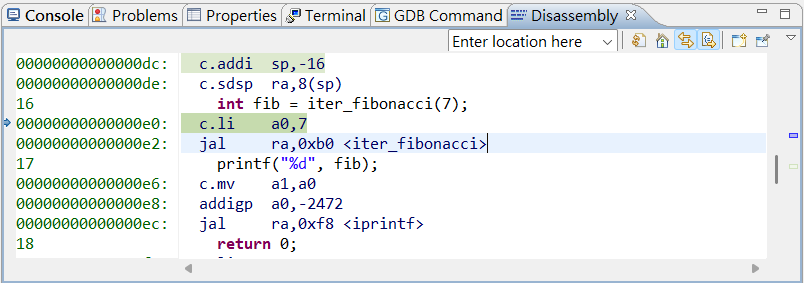
\includegraphics[width=0.4\textwidth]{img/iter_reference.png} & 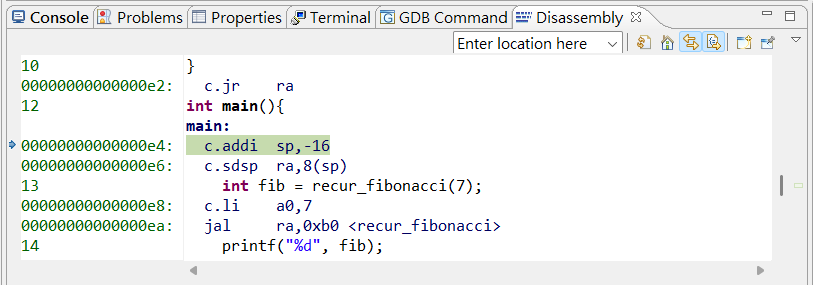
\includegraphics[width=0.4\textwidth]{img/recur_reference.png} \\
    \hline
    starting memory address & 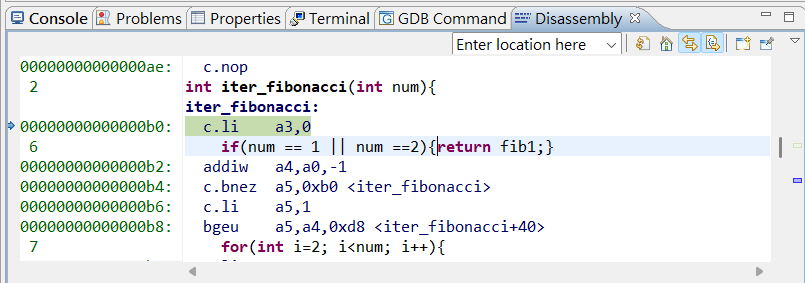
\includegraphics[width=0.4\textwidth]{img/iter_start.png} & 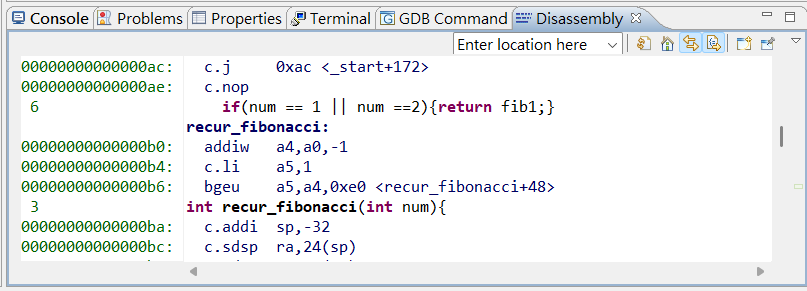
\includegraphics[width=0.4\textwidth]{img/recur_start.png} \\
    \hline
    ending memory address & 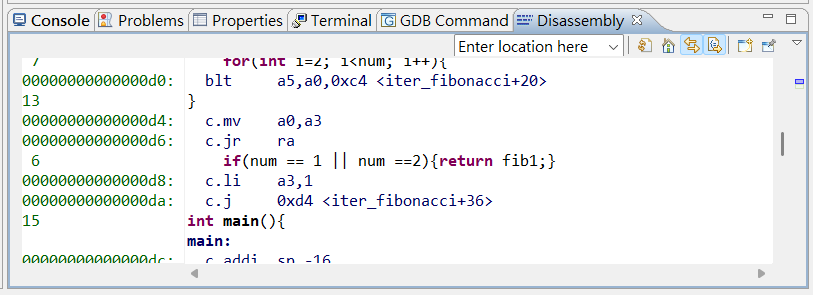
\includegraphics[width=0.4\textwidth]{img/iter_end.png} & 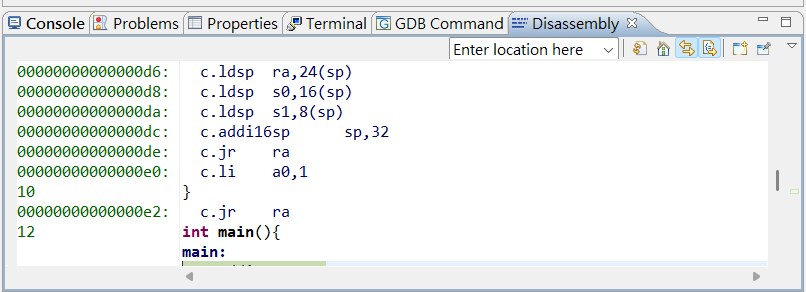
\includegraphics[width=0.4\textwidth]{img/recur_end.png} \\
    \hline
    \end{tabular}
\end{table}

\subsection*{(b)}

\begin{table}[H]
    \centering
    \begin{tabular}{|l|c|c|c|c|}
    \hline
    \multirow{2}{*}{Function Name} & \multicolumn{2}{c|}{Argument \textbf{num}} & \multicolumn{2}{c|}{Return Value} \\
    \cline{2-5}
    & Register Name & Value & Register Name & Value \\
    \hline
    \textbf{iter\_fibonacci} & a0 & 7 & a0 & 13 \\
    \hline
    \textbf{recur\_fibonacci} & a0 & 7 & a0 & 13 \\
    \hline
    \end{tabular}
\end{table}

\begin{table}[H]
    \centering
    \begin{tabular}{|c|c|}
    \hline
    \textbf{iter} & \textbf{recur} \\
    \hline
    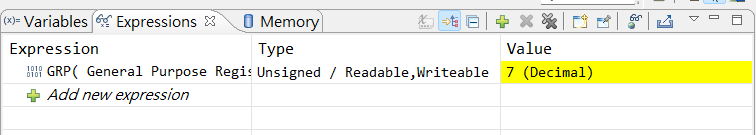
\includegraphics[width=0.4\textwidth]{img/iter_argument.png} & 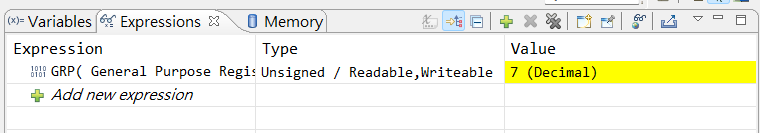
\includegraphics[width=0.4\textwidth]{img/recur_argument.png} \\
    \hline
    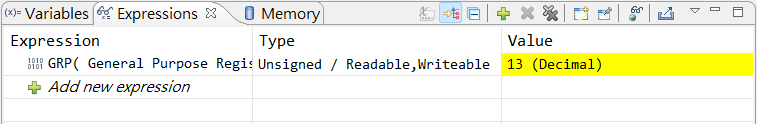
\includegraphics[width=0.4\textwidth]{img/iter_return.png} & 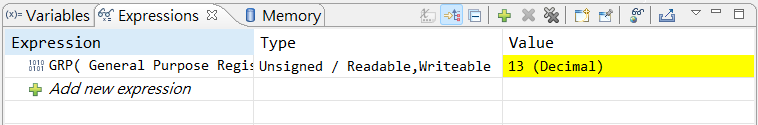
\includegraphics[width=0.4\textwidth]{img/recur_return.png} \\
    \hline
    \end{tabular}
\end{table}

\subsection*{(c)}

\begin{figure}[H]
    \centering
    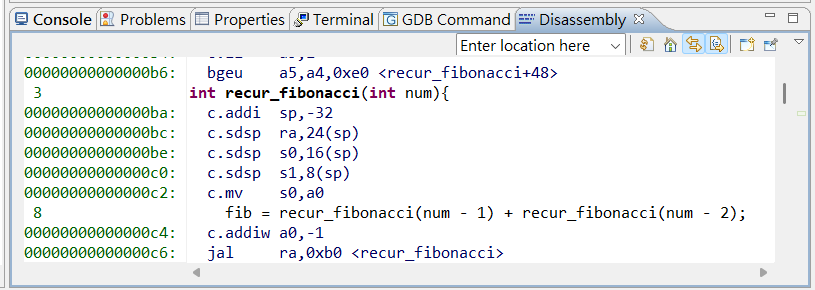
\includegraphics[width=0.6\textwidth]{img/stack_layout.png}
\end{figure}

\begin{table}[H]
    \centering
    \begin{tabular}{|c|c|c|c|}
    \hline
    Memory Address & Instruction & Saved Registers & Stack Offset \\
    \hline
    0x0000 0000 0000 00c0 & c.sdsp s1,8(sp) & s1 & 8 \\
    \hline
    0x0000 0000 0000 00be & c.sdsp s0,16(sp) & s0 & 16 \\
    \hline
    \end{tabular}
\end{table}

Note that \texttt{ra} is preserved by the caller, so it is excluded from the table.

\subsection*{(d)}

To calculate the smallest memory address reached by the stack pointer during \textbf{recur\_fibonacci()} function calls, we need to analyze the recursion pattern:

\begin{align*}
\texttt{recur\_fibonacci}(7) &= \texttt{recur\_fibonacci}(6) + \texttt{recur\_fibonacci}(5) \\
&= \texttt{recur\_fibonacci}(5) + \texttt{recur\_fibonacci}(4) + \ldots \\
&= \texttt{recur\_fibonacci}(4) + \texttt{recur\_fibonacci}(3) + \ldots \\
&= \texttt{recur\_fibonacci}(3) + \texttt{recur\_fibonacci}(2) + \ldots \\
&= \texttt{recur\_fibonacci}(2) + \texttt{recur\_fibonacci}(1) + \ldots \\
&= 1 + 1 + \ldots
\end{align*}

When initially entering \textbf{recur\_fibonacci()}, the stack pointer value is \texttt{0x0000 0000 02FF FFF0}. With each recursive call consuming 32 bytes of stack space and a maximum recursion depth of 5 levels, the smallest memory address the stack pointer will reach is:
$$\texttt{0x0000 0000 02FF FFF0} - (32 \times 5) = \texttt{0x0000 0000 02FF FF50}$$

\subsection*{(e)}

\subsubsection*{(i)}

\begin{table}[H]
    \centering
    \begin{tabular}{|c|p{4.5cm}|p{6.5cm}|}
    \hline
    \textbf{Code Memory Address} & \textbf{Instruction} & \textbf{Explanation} \\
    \hline
    0x0000 0000 0000 00b0 & \texttt{addiw a4, a0, -1} & Subtract 1 from input parameter \texttt{num} (in \texttt{a0}) and store \texttt{num-1} in \texttt{a4}. This is the first step in checking for the Fibonacci base case. \\
    \hline
    0x0000 0000 0000 00b4 & \texttt{c.li a5, 1} & Load immediate value 1 into register \texttt{a5} for comparison. \\
    \hline
    0x0000 0000 0000 00b6 & \texttt{bgeu a5, a4, 0xe0 <recur\_fibonacci+48>} & Branch if \texttt{a5 >= a4}, meaning if \texttt{1 >= num-1}, which is equivalent to \texttt{num <= 2}. This identifies the base case where \texttt{F(1) = F(2) = 1}. \\
    \hline
    0x0000 0000 0000 00e0 & \texttt{c.li a0, 1} & Load immediate value 1 into register \texttt{a0} for the return value of the base case. \\
    \hline
    0x0000 0000 0000 00e2 & \texttt{c.jr ra} & Jump to the return address stored in \texttt{ra}. \\
    \hline
    \end{tabular}
\end{table}

\begin{figure}[H]
    \centering
    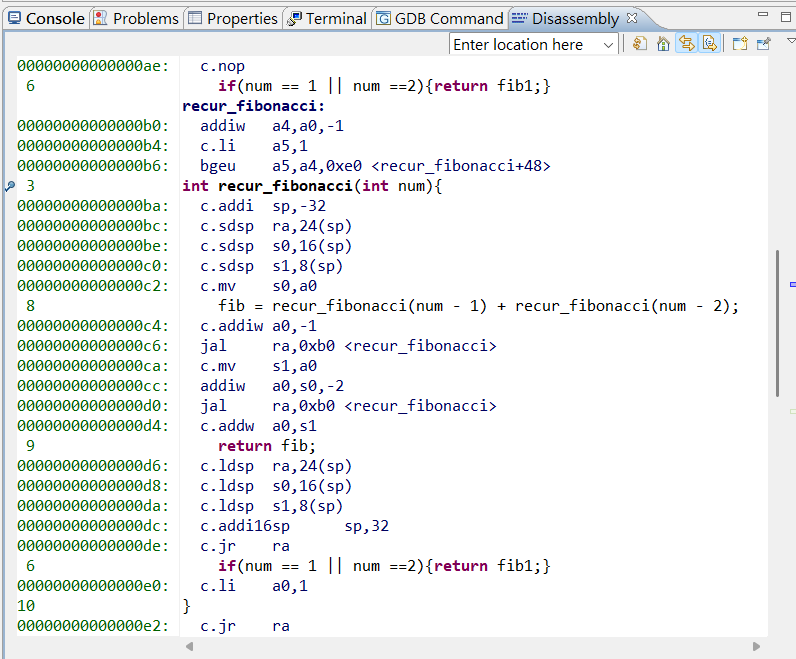
\includegraphics[width=0.6\textwidth]{img/base_case.png}
\end{figure}

\subsubsection*{(ii)}
Yes, it is possible to optimize the Assembly code for the base case check in \textbf{recur\_fibonacci()}.

Optimized implementation:
\begin{lstlisting}[basicstyle=\ttfamily\small, numbers=left, numberstyle=\tiny\color{gray}, stepnumber=1, frame=single]
c.li a5, 3                         # Load immediate 3 into a5
bltu a0, a5, 0xe0 <recur_fibonacci+48>  # Branch if num < 3
c.li a0, 1                         # Load immediate 1 into a0 (return value)
c.jr ra                            # Jump to return address
\end{lstlisting}

This optimization eliminates the subtraction operation and directly compares the input parameter.

\section*{2}

\subsection*{(a)}

\begin{longtable}{|c|l|p{9cm}|}
    \hline
    \textbf{\texttt{Address}} & \textbf{texttt{Instruction}} & \textbf{\texttt{Updated Register / Memory}} \\
    \hline
    \endhead

    \hline
    \endfoot

    \hline
    \endlastfoot

    \texttt{0x0000 0000 0003 0098} & \texttt{add x29, x30, x31} & \texttt{x29} ← \texttt{0x0000 0000 0000 10AA} \\
    \hline
    \texttt{0x0000 0000 0003 009C} & \texttt{sw x29, -4(x3)} & \texttt{MEM[0x0000 002E 0040 0014]} = \texttt{0x0000 10AA} \\
    \hline
    \texttt{0x0000 0000 0003 00A0} & \texttt{add x0, x12, x14} & Nothing (\texttt{x0} is immutable) \\
    \hline
    \texttt{0x0000 0000 0003 00A4} & \texttt{sll x12, x12, x5} & \texttt{x12} ← \texttt{x12} << 31 = \texttt{0x99F8 0050 0000 0000} \\
    \hline
    \texttt{0x0000 0000 0003 00A8} & \texttt{bge x12, x15, GE} & (Nothing) \\
    \hline
    \texttt{0x0000 0000 0003 00AC} & \texttt{jalr x1, 0(x3)} & \texttt{x1} ← \texttt{PC} + 4 = \texttt{0x0000 0000 0003 00B0} \\
    \hline
    \texttt{0x0000 002E 0040 0018} & \texttt{lb x12, -7(x3)} & \texttt{x12} ← \texttt{0xFFFF FFFF FFFF FFCC} (sign-extension) \\
    \hline
    \texttt{0x0000 002E 0040 001C} & \texttt{and x12, x12, x13} & \texttt{x12} ← \texttt{0x0000 0000 0000 00C0} \\
    \hline
    \texttt{0x0000 002E 0040 0020} & \texttt{sb x12, 30(x3)} & \texttt{MEM[0x0000 002E 0040 0034]} = \texttt{0x00C0 8067} \\
    \hline
    \texttt{0x0000 002E 0040 0024} & \texttt{lw x12, 24(x3)} & \texttt{x12} ← \texttt{0x0000 0000 4042 05B3} \\
    \hline
    \texttt{0x0000 002E 0040 0028} & \texttt{xor x12, x14, x12} & \texttt{x12} ← \texttt{0x0000 0000 0052 87B3} \\
    \hline
    \texttt{0x0000 002E 0040 002C} & \texttt{sw x12, 24(x3)} & \texttt{MEM[0x0000 002E 0040 0030]} = \texttt{0x0052 87B3} \\
    \hline
    \texttt{0x0000 002E 0040 0030} & \texttt{add x15, x5, x5} & \texttt{x15} ← \texttt{0x0000 0000 0000 003E} \\
    \hline
    \texttt{0x0000 002E 0040 0034} & \texttt{jalr x0, 12(x1)} & (Nothing) \\
    \hline
    \texttt{0x0000 0000 0003 00BC} & \texttt{sra x18, x18, x5} & \texttt{x18} ← \texttt{0xFFFF FFFF 7510 EEA2} \\
    \hline
    \texttt{0x0000 0000 0003 00C0} & \texttt{lb x19, -6(x3)} & \texttt{x19} ← \texttt{0xFFFF FFFF FFFF FF83} \\
    \hline
    \texttt{0x0000 0000 0003 00C4} & \texttt{sd x19, -8(x3)} & \begin{tabular}[t]{@{}l@{}}
                                                \texttt{MEM[0x0000 002E 0040 0010]} = \texttt{0xFFFF FF83} \\
                                                \texttt{MEM[0x0000 002E 0040 0014]} = \texttt{0xFFFF FFFF}
                                            \end{tabular} \\
    \hline
\end{longtable}

\subsection*{(b)}

Numbers of memory accesses:
\begin{itemize}
    \item Instruction fetches: 15
    \item Load operations: 3
    \item Store operations: 3
\end{itemize}

So the total number of memory accesses is $15 + 3 + 3 = 21$.

\subsection*{(c)}

We notice that the target address $\texttt{0x0000 0000 1F03 00C4}$ can be expressed as:

$$\texttt{0x1F03 00C4} = \texttt{0x0003 00C8} + \texttt{0x1F00 0000} - \texttt{0x0000 0004}$$

So we can use auipc first to load the upper 20 bits of the address, and then use jalr to jump to the target address.

\begin{lstlisting}[basicstyle=\ttfamily\small, numbers=left, numberstyle=\tiny\color{gray}, stepnumber=1, frame=single]
auipc x5, 0x1F000    # x5 ← PC + 0x1F000000
jalr x0, -4(x5)      # Jump to x5 - 4 (target: 0x0000 0000 1F03 00C4)
\end{lstlisting}

\section*{3}
The overall code implements the Z algorithm for pattern matching. The missing C code contains the logic for updating array B based on previously computed values. The missing RISC-V instruction segment contains the implementation that updates arrays A and B within the main computation loop of the algorithm.

\subsection*{(a)}

The missing C code is:
\begin{lstlisting}[language=C++, basicstyle=\ttfamily\small, keywordstyle=\color{blue}\bfseries, commentstyle=\color{gray}\itshape, stringstyle=\color{red}, numbers=left, numberstyle=\tiny\color{gray}, stepnumber=1, frame=single]
int l = 0;
int r = 0;
int i = 0;
for (; i < n; ++i) {
    // missing C code
    if (i < r) {
        int k = i - l;
        if (r - i < B[k]) {
            B[i] = r - i;
        } else {
            B[i] = B[k];
        }
    }
    // end of missing C code
}
\end{lstlisting}

\subsection*{(b)}

The missing RISC-V Instruction is:
\begin{lstlisting}[basicstyle=\ttfamily\small, numbers=left, numberstyle=\tiny\color{gray}, stepnumber=1, frame=single]
LOOP2:
# --------------- missing RISC-V instruction ---------------
    lw x15, 0(x11)     # x15 ← B[i]
    add x16, x10, x15  # x16 ← i + B[i]
    bge x16, x7, B2    # if (i + B[i] >= n) goto B2
    slli x17, x15, 2   # x17 ← B[i] << 2
    add x17, x15, x17  # x17 ← &A[B[i]]
    lw x17, 0(x17)     # x17 ← A[B[i]]
    slli x18, x16, 2   # x18 ← (i + B[i]) << 2
    add x18, x5, x18   # x18 ← &A[i + B[i]]
    lw x18, 0(x18)     # x18 ← A[i + B[i]]
    bne x17, x18, B2   # if (A[B[i]] != A[i + B[i]]) goto B2
    addi x15, x15, 1   # B[i]++
    sw x15, 0(x11)     # B[i] ← x15 (store back to memory)
    jal x0, LOOP2      # goto LOOP2
B2:
    bge x29, x16, B3   # if (i + B[i] <= r) goto B3
    addi x28, x10, 0   # l ← i
    addi x29, x16, 0   # r ← i + B[i]
B3:
# --------------- end of missing RISC-V instruction ---------------
    addi x10, x10, 1   # i++
    jal x0, LOOP1      # goto LOOP1
\end{lstlisting}

\section*{4}

\begin{lstlisting}[basicstyle=\ttfamily\small, numbers=left, numberstyle=\tiny\color{gray}, stepnumber=1, frame=single]
Func:
    # Allocate stack frame for ra, s0, s1, s2 (total 32 bytes)
    addi x2, x2, -32        # sp ← sp - 32
    sd   x1, 24(x2)         # save return address
    sd   x8, 16(x2)         # save s0
    sd   x9, 8(x2)          # save s1
    sd   x18, 0(x2)         # save s2

    add  x8, x0, x10        # x8 ← x10 (save n to s0)

    # Base case: if (n <= 1) return 1
    addi x5, x0, 1          # x5 ← 1
    blt  x5, x8, L0         # if n > 1, goto L0
    addi x10, x0, 1         # x10 ← 1 (return value)
    jalr x0, 0(x1)          # return

L0:
    addi x9, x0, 0          # x9 ← i = 0
    addi x18, x0, 0         # x18 ← res = 0

LOOP:
    bge  x9, x8, DONE       # if i >= n, goto DONE

    # Call Func(i)
    add  x10, x0, x9        # argument = i
    jal  x1, Func
    add  x6, x0, x10        # x6 ← Func(i)

    # Call Func(n - i - 1)
    sub  x7, x8, x9         # x7 ← n - i
    addi x7, x7, -1         # x7 ← n - i - 1
    add  x10, x0, x7        # argument = n - i - 1
    jal  x1, Func
    mul  x6, x6, x10        # x6 ← Func(i) * Func(n - i - 1)
    add  x18, x18, x6       # res += Func(i) * Func(n - i - 1)

    addi x9, x9, 1          # i++
    beq  x0, x0, LOOP       # unconditional jump to LOOP

DONE:
    add  x10, x0, x18       # return res

    # Restore ra, s0, s1, s2
    ld   x18, 0(x2)         # restore s2
    ld   x9,  8(x2)         # restore s1
    ld   x8, 16(x2)         # restore s0
    ld   x1, 24(x2)         # restore return address
    addi x2, x2, 32         # deallocate stack
    jalr x0, 0(x1)          # return
\end{lstlisting}

\end{document}